% Options for packages loaded elsewhere
\PassOptionsToPackage{unicode}{hyperref}
\PassOptionsToPackage{hyphens}{url}
\PassOptionsToPackage{dvipsnames,svgnames,x11names}{xcolor}
%
\documentclass[
  10pt,
]{article}
\title{RNA-seq course- week1}
\author{Serhiy Naumenko}
\date{2023-09-30}

\usepackage{amsmath,amssymb}
\usepackage{lmodern}
\usepackage{iftex}
\ifPDFTeX
  \usepackage[T1]{fontenc}
  \usepackage[utf8]{inputenc}
  \usepackage{textcomp} % provide euro and other symbols
\else % if luatex or xetex
  \usepackage{unicode-math}
  \defaultfontfeatures{Scale=MatchLowercase}
  \defaultfontfeatures[\rmfamily]{Ligatures=TeX,Scale=1}
  \setmainfont[]{Tempora}
\fi
% Use upquote if available, for straight quotes in verbatim environments
\IfFileExists{upquote.sty}{\usepackage{upquote}}{}
\IfFileExists{microtype.sty}{% use microtype if available
  \usepackage[]{microtype}
  \UseMicrotypeSet[protrusion]{basicmath} % disable protrusion for tt fonts
}{}
\makeatletter
\@ifundefined{KOMAClassName}{% if non-KOMA class
  \IfFileExists{parskip.sty}{%
    \usepackage{parskip}
  }{% else
    \setlength{\parindent}{0pt}
    \setlength{\parskip}{6pt plus 2pt minus 1pt}}
}{% if KOMA class
  \KOMAoptions{parskip=half}}
\makeatother
\usepackage{xcolor}
\IfFileExists{xurl.sty}{\usepackage{xurl}}{} % add URL line breaks if available
\IfFileExists{bookmark.sty}{\usepackage{bookmark}}{\usepackage{hyperref}}
\hypersetup{
  pdftitle={RNA-seq course- week1},
  pdfauthor={Serhiy Naumenko},
  colorlinks=true,
  linkcolor={Maroon},
  filecolor={Maroon},
  citecolor={Blue},
  urlcolor={blue},
  pdfcreator={LaTeX via pandoc}}
\urlstyle{same} % disable monospaced font for URLs
\usepackage[margin=1in]{geometry}
\usepackage{color}
\usepackage{fancyvrb}
\newcommand{\VerbBar}{|}
\newcommand{\VERB}{\Verb[commandchars=\\\{\}]}
\DefineVerbatimEnvironment{Highlighting}{Verbatim}{commandchars=\\\{\}}
% Add ',fontsize=\small' for more characters per line
\usepackage{framed}
\definecolor{shadecolor}{RGB}{248,248,248}
\newenvironment{Shaded}{\begin{snugshade}}{\end{snugshade}}
\newcommand{\AlertTok}[1]{\textcolor[rgb]{0.94,0.16,0.16}{#1}}
\newcommand{\AnnotationTok}[1]{\textcolor[rgb]{0.56,0.35,0.01}{\textbf{\textit{#1}}}}
\newcommand{\AttributeTok}[1]{\textcolor[rgb]{0.77,0.63,0.00}{#1}}
\newcommand{\BaseNTok}[1]{\textcolor[rgb]{0.00,0.00,0.81}{#1}}
\newcommand{\BuiltInTok}[1]{#1}
\newcommand{\CharTok}[1]{\textcolor[rgb]{0.31,0.60,0.02}{#1}}
\newcommand{\CommentTok}[1]{\textcolor[rgb]{0.56,0.35,0.01}{\textit{#1}}}
\newcommand{\CommentVarTok}[1]{\textcolor[rgb]{0.56,0.35,0.01}{\textbf{\textit{#1}}}}
\newcommand{\ConstantTok}[1]{\textcolor[rgb]{0.00,0.00,0.00}{#1}}
\newcommand{\ControlFlowTok}[1]{\textcolor[rgb]{0.13,0.29,0.53}{\textbf{#1}}}
\newcommand{\DataTypeTok}[1]{\textcolor[rgb]{0.13,0.29,0.53}{#1}}
\newcommand{\DecValTok}[1]{\textcolor[rgb]{0.00,0.00,0.81}{#1}}
\newcommand{\DocumentationTok}[1]{\textcolor[rgb]{0.56,0.35,0.01}{\textbf{\textit{#1}}}}
\newcommand{\ErrorTok}[1]{\textcolor[rgb]{0.64,0.00,0.00}{\textbf{#1}}}
\newcommand{\ExtensionTok}[1]{#1}
\newcommand{\FloatTok}[1]{\textcolor[rgb]{0.00,0.00,0.81}{#1}}
\newcommand{\FunctionTok}[1]{\textcolor[rgb]{0.00,0.00,0.00}{#1}}
\newcommand{\ImportTok}[1]{#1}
\newcommand{\InformationTok}[1]{\textcolor[rgb]{0.56,0.35,0.01}{\textbf{\textit{#1}}}}
\newcommand{\KeywordTok}[1]{\textcolor[rgb]{0.13,0.29,0.53}{\textbf{#1}}}
\newcommand{\NormalTok}[1]{#1}
\newcommand{\OperatorTok}[1]{\textcolor[rgb]{0.81,0.36,0.00}{\textbf{#1}}}
\newcommand{\OtherTok}[1]{\textcolor[rgb]{0.56,0.35,0.01}{#1}}
\newcommand{\PreprocessorTok}[1]{\textcolor[rgb]{0.56,0.35,0.01}{\textit{#1}}}
\newcommand{\RegionMarkerTok}[1]{#1}
\newcommand{\SpecialCharTok}[1]{\textcolor[rgb]{0.00,0.00,0.00}{#1}}
\newcommand{\SpecialStringTok}[1]{\textcolor[rgb]{0.31,0.60,0.02}{#1}}
\newcommand{\StringTok}[1]{\textcolor[rgb]{0.31,0.60,0.02}{#1}}
\newcommand{\VariableTok}[1]{\textcolor[rgb]{0.00,0.00,0.00}{#1}}
\newcommand{\VerbatimStringTok}[1]{\textcolor[rgb]{0.31,0.60,0.02}{#1}}
\newcommand{\WarningTok}[1]{\textcolor[rgb]{0.56,0.35,0.01}{\textbf{\textit{#1}}}}
\usepackage{graphicx}
\makeatletter
\def\maxwidth{\ifdim\Gin@nat@width>\linewidth\linewidth\else\Gin@nat@width\fi}
\def\maxheight{\ifdim\Gin@nat@height>\textheight\textheight\else\Gin@nat@height\fi}
\makeatother
% Scale images if necessary, so that they will not overflow the page
% margins by default, and it is still possible to overwrite the defaults
% using explicit options in \includegraphics[width, height, ...]{}
\setkeys{Gin}{width=\maxwidth,height=\maxheight,keepaspectratio}
% Set default figure placement to htbp
\makeatletter
\def\fps@figure{htbp}
\makeatother
\setlength{\emergencystretch}{3em} % prevent overfull lines
\providecommand{\tightlist}{%
  \setlength{\itemsep}{0pt}\setlength{\parskip}{0pt}}
\setcounter{secnumdepth}{5}
\ifLuaTeX
  \usepackage{selnolig}  % disable illegal ligatures
\fi

\begin{document}
\maketitle

{
\hypersetup{linkcolor=}
\setcounter{tocdepth}{2}
\tableofcontents
}
\hypertarget{overview}{%
\section{Overview}\label{overview}}

\begin{itemize}
\tightlist
\item
  Negative binomial distribution
\item
  Від'ємний біноміальний розподіл
\item
  \url{https://rpubs.com/mpfoley73/458738}
\item
  \url{https://uk.wikipedia.org/wiki/Від'ємний_біноміальний_розподіл}
\item
  \url{https://www.youtube.com/watch?v=lJw6Ku_jQkM}
\end{itemize}

\newpage

\begin{Shaded}
\begin{Highlighting}[]
\NormalTok{r }\OtherTok{\textless{}{-}}  \DecValTok{3} \CommentTok{\# n success}
\NormalTok{p }\OtherTok{\textless{}{-}}  \FloatTok{0.20} \CommentTok{\# success}
\NormalTok{n }\OtherTok{\textless{}{-}}  \DecValTok{7} \SpecialCharTok{{-}}\NormalTok{ r }\CommentTok{\# failures}
\CommentTok{\# exact}
\FunctionTok{dnbinom}\NormalTok{(}\AttributeTok{x =}\NormalTok{ n, }\AttributeTok{size =}\NormalTok{ r, }\AttributeTok{prob =}\NormalTok{ p)}
\end{Highlighting}
\end{Shaded}

\begin{verbatim}
## [1] 0.049152
\end{verbatim}

\begin{Shaded}
\begin{Highlighting}[]
\CommentTok{\# simulated}
\FunctionTok{mean}\NormalTok{(}\FunctionTok{rnbinom}\NormalTok{(}\AttributeTok{n =} \DecValTok{10000}\NormalTok{, }\AttributeTok{size =}\NormalTok{ r, }\AttributeTok{prob =}\NormalTok{ p) }\SpecialCharTok{==}\NormalTok{ n)}
\end{Highlighting}
\end{Shaded}

\begin{verbatim}
## [1] 0.0485
\end{verbatim}

\newpage

\begin{Shaded}
\begin{Highlighting}[]
\NormalTok{r }\OtherTok{\textless{}{-}} \DecValTok{3}
\NormalTok{p }\OtherTok{\textless{}{-}} \FloatTok{0.20}

\NormalTok{sim\_nb }\OtherTok{\textless{}{-}} \FunctionTok{data.frame}\NormalTok{(}\AttributeTok{x =} \DecValTok{0}\SpecialCharTok{:}\DecValTok{20}\NormalTok{, }\AttributeTok{prob =} \FunctionTok{dnbinom}\NormalTok{(}\AttributeTok{x =} \DecValTok{0}\SpecialCharTok{:}\DecValTok{20}\NormalTok{, }\AttributeTok{size =}\NormalTok{ r, }\AttributeTok{prob =}\NormalTok{ p)) }\SpecialCharTok{\%\textgreater{}\%}
  \FunctionTok{mutate}\NormalTok{(}\AttributeTok{Failures =} \FunctionTok{ifelse}\NormalTok{(x }\SpecialCharTok{==}\NormalTok{ n, n, }\StringTok{"other"}\NormalTok{)) }

\CommentTok{\# NB: factor}

\NormalTok{sim\_nb }\SpecialCharTok{\%\textgreater{}\%}
\FunctionTok{ggplot}\NormalTok{(}\FunctionTok{aes}\NormalTok{(}\AttributeTok{x =} \FunctionTok{factor}\NormalTok{(x), }\AttributeTok{y =}\NormalTok{ prob, }\AttributeTok{fill =}\NormalTok{ Failures)) }\SpecialCharTok{+}
  \FunctionTok{geom\_col}\NormalTok{() }\SpecialCharTok{+}
  \FunctionTok{geom\_text}\NormalTok{(}
    \FunctionTok{aes}\NormalTok{(}\AttributeTok{label =} \FunctionTok{round}\NormalTok{(prob,}\DecValTok{2}\NormalTok{), }\AttributeTok{y =}\NormalTok{ prob }\SpecialCharTok{+} \FloatTok{0.01}\NormalTok{),}
    \AttributeTok{position =} \FunctionTok{position\_dodge}\NormalTok{(}\FloatTok{0.9}\NormalTok{),}
    \AttributeTok{size =} \DecValTok{3}\NormalTok{,}
    \AttributeTok{vjust =} \DecValTok{0}
\NormalTok{  ) }\SpecialCharTok{+}
  \FunctionTok{labs}\NormalTok{(}\AttributeTok{title =} \StringTok{"Probability of r = 3 Successes in X = 7 Trials"}\NormalTok{,}
       \AttributeTok{subtitle =} \StringTok{"NB(3,.2)"}\NormalTok{,}
       \AttributeTok{x =} \StringTok{"Failed Trials (X {-} r)"}\NormalTok{,}
       \AttributeTok{y =} \StringTok{"Probability"}\NormalTok{)  }\SpecialCharTok{+}
  \FunctionTok{geom\_vline}\NormalTok{(}\AttributeTok{xintercept =}\NormalTok{ r}\SpecialCharTok{*}\NormalTok{(}\DecValTok{1}\SpecialCharTok{{-}}\NormalTok{p)}\SpecialCharTok{/}\NormalTok{p, }\AttributeTok{linetype =} \StringTok{"dashed"}\NormalTok{, }\AttributeTok{color =} \StringTok{"red"}\NormalTok{)}
\end{Highlighting}
\end{Shaded}

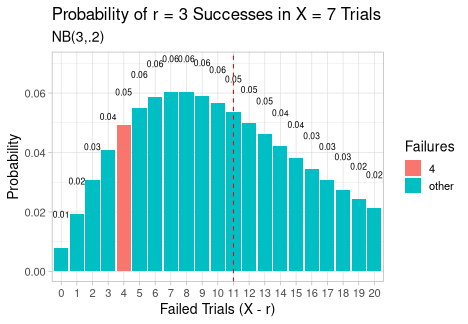
\includegraphics{06.negative_binomial_files/figure-latex/unnamed-chunk-4-1.png}
\# Expected number of trials

\begin{Shaded}
\begin{Highlighting}[]
\NormalTok{r }\OtherTok{\textless{}{-}}  \DecValTok{3} \CommentTok{\# success}
\NormalTok{p }\OtherTok{\textless{}{-}}  \FloatTok{0.20}
\CommentTok{\# mean}
\CommentTok{\# exact}
\NormalTok{r }\SpecialCharTok{/}\NormalTok{ p}
\end{Highlighting}
\end{Shaded}

\begin{verbatim}
## [1] 15
\end{verbatim}

\begin{itemize}
\tightlist
\item
  Mean = 12`
\item
  Var = 60
\end{itemize}

\hypertarget{simulated}{%
\section{Simulated}\label{simulated}}

\begin{Shaded}
\begin{Highlighting}[]
\FunctionTok{var}\NormalTok{(}\FunctionTok{rnbinom}\NormalTok{(}\AttributeTok{n =} \DecValTok{100000}\NormalTok{, }\AttributeTok{size =}\NormalTok{ r, }\AttributeTok{prob =}\NormalTok{ p))}
\end{Highlighting}
\end{Shaded}

\begin{verbatim}
## [1] 59.03792
\end{verbatim}

\hypertarget{cumulative-probability}{%
\section{Cumulative probability}\label{cumulative-probability}}

\begin{Shaded}
\begin{Highlighting}[]
\FunctionTok{data.frame}\NormalTok{(}\AttributeTok{x =} \DecValTok{1}\SpecialCharTok{:}\DecValTok{20}\NormalTok{, }
           \AttributeTok{pmf =} \FunctionTok{dnbinom}\NormalTok{(}\AttributeTok{x =} \DecValTok{1}\SpecialCharTok{:}\DecValTok{20}\NormalTok{, }\AttributeTok{size =}\NormalTok{ r, }\AttributeTok{prob =}\NormalTok{ p),}
           \AttributeTok{cdf =} \FunctionTok{pnbinom}\NormalTok{(}\AttributeTok{q =} \DecValTok{1}\SpecialCharTok{:}\DecValTok{20}\NormalTok{, }\AttributeTok{size =}\NormalTok{ r, }\AttributeTok{prob =}\NormalTok{ p, }\AttributeTok{lower.tail =} \ConstantTok{TRUE}\NormalTok{)) }\SpecialCharTok{\%\textgreater{}\%}
\FunctionTok{ggplot}\NormalTok{(}\FunctionTok{aes}\NormalTok{(}\AttributeTok{x =} \FunctionTok{factor}\NormalTok{(x), }\AttributeTok{y =}\NormalTok{ cdf)) }\SpecialCharTok{+}
  \FunctionTok{geom\_col}\NormalTok{() }\SpecialCharTok{+}
  \FunctionTok{geom\_text}\NormalTok{(}
    \FunctionTok{aes}\NormalTok{(}\AttributeTok{label =} \FunctionTok{round}\NormalTok{(cdf,}\DecValTok{2}\NormalTok{), }\AttributeTok{y =}\NormalTok{ cdf }\SpecialCharTok{+} \FloatTok{0.01}\NormalTok{),}
    \AttributeTok{position =} \FunctionTok{position\_dodge}\NormalTok{(}\FloatTok{0.9}\NormalTok{),}
    \AttributeTok{size =} \DecValTok{3}\NormalTok{,}
    \AttributeTok{vjust =} \DecValTok{0}
\NormalTok{  ) }\SpecialCharTok{+}
  \FunctionTok{labs}\NormalTok{(}\AttributeTok{title =} \StringTok{"Cumulative Probability of X = x failed trials to achieve 3rd success"}\NormalTok{,}
       \AttributeTok{subtitle =} \StringTok{"NB(3,.2)"}\NormalTok{,}
       \AttributeTok{x =} \StringTok{"Failed Trials (x)"}\NormalTok{,}
       \AttributeTok{y =} \StringTok{"probability"}\NormalTok{) }
\end{Highlighting}
\end{Shaded}

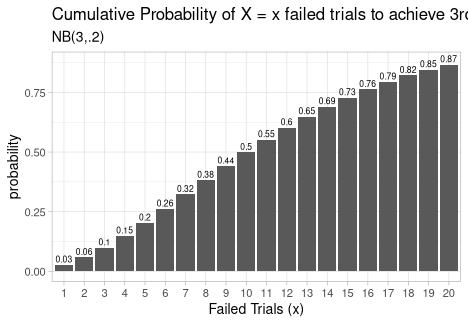
\includegraphics{06.negative_binomial_files/figure-latex/unnamed-chunk-7-1.png}

\hypertarget{sessioninfo}{%
\section{sessionInfo()}\label{sessioninfo}}

\begin{Shaded}
\begin{Highlighting}[]
\FunctionTok{sessionInfo}\NormalTok{()}
\end{Highlighting}
\end{Shaded}

\begin{verbatim}
## R version 4.2.2 (2022-10-31)
## Platform: x86_64-redhat-linux-gnu (64-bit)
## Running under: Fedora Linux 37 (Workstation Edition)
## 
## Matrix products: default
## BLAS/LAPACK: /usr/lib64/libflexiblas.so.3.3
## 
## locale:
##  [1] LC_CTYPE=en_US.UTF-8       LC_NUMERIC=C              
##  [3] LC_TIME=en_US.UTF-8        LC_COLLATE=en_US.UTF-8    
##  [5] LC_MONETARY=en_US.UTF-8    LC_MESSAGES=en_US.UTF-8   
##  [7] LC_PAPER=en_US.UTF-8       LC_NAME=C                 
##  [9] LC_ADDRESS=C               LC_TELEPHONE=C            
## [11] LC_MEASUREMENT=en_US.UTF-8 LC_IDENTIFICATION=C       
## 
## attached base packages:
## [1] stats     graphics  grDevices utils     datasets  methods   base     
## 
## other attached packages:
##  [1] knitr_1.41        mosaic_1.8.4.2    mosaicData_0.20.3 ggformula_0.10.4 
##  [5] Matrix_1.6-1      lattice_0.20-45   forcats_0.5.2     stringr_1.5.0    
##  [9] dplyr_1.0.10      purrr_1.0.0       readr_2.1.3       tidyr_1.2.1      
## [13] tibble_3.1.8      ggplot2_3.4.0     tidyverse_1.3.2  
## 
## loaded via a namespace (and not attached):
##  [1] httr_1.4.4          jsonlite_1.8.4      modelr_0.1.10      
##  [4] assertthat_0.2.1    highr_0.10          googlesheets4_1.0.1
##  [7] ggstance_0.3.6      cellranger_1.1.0    yaml_2.3.6         
## [10] pillar_1.8.1        backports_1.4.1     glue_1.6.2         
## [13] digest_0.6.31       polyclip_1.10-4     rvest_1.0.3        
## [16] colorspace_2.0-3    htmltools_0.5.4     pkgconfig_2.0.3    
## [19] broom_1.0.2         labelled_2.12.0     haven_2.5.1        
## [22] scales_1.2.1        tweenr_2.0.2        tzdb_0.3.0         
## [25] ggforce_0.4.1       timechange_0.1.1    googledrive_2.0.0  
## [28] generics_0.1.3      farver_2.1.1        ellipsis_0.3.2     
## [31] withr_2.5.0         cli_3.5.0           magrittr_2.0.3     
## [34] crayon_1.5.2        readxl_1.4.1        evaluate_0.19      
## [37] fs_1.5.2            fansi_1.0.3         MASS_7.3-58.1      
## [40] xml2_1.3.3          tools_4.2.2         hms_1.1.2          
## [43] gargle_1.2.0        lifecycle_1.0.3     munsell_0.5.0      
## [46] reprex_2.0.2        compiler_4.2.2      rlang_1.0.6        
## [49] grid_4.2.2          ggridges_0.5.4      rstudioapi_0.14    
## [52] mosaicCore_0.9.2.1  labeling_0.4.2      rmarkdown_2.19     
## [55] gtable_0.3.1        DBI_1.1.3           R6_2.5.1           
## [58] lubridate_1.9.0     fastmap_1.1.0       utf8_1.2.2         
## [61] stringi_1.7.8       Rcpp_1.0.9          vctrs_0.5.1        
## [64] dbplyr_2.2.1        tidyselect_1.2.0    xfun_0.36
\end{verbatim}

\end{document}
